
\section{todo Genetic programming}

Genetic programming (GP) is an evolutionary machine learning approach that can automatically generate and improve programs to solve a problem.
For this purpose, the best programs are selected from randomly generated candidates of a population. The selected candidates can be mutated and crossed to become better and better over generations.

\subsection{TODO Genetic Generations, populations}

The goal of GP is to find the one program over many generations that is better than all the others. To find this program, the population of programs must both promote the best programs and create space for new approaches. (todo Exploration-exploitation tradeoff?) For this purpose, both the selection and the genetic modifications must be chosen accordingly.

\subsection{TODO2 Genetic Selection (Tournament Selection)}
    
In order to achieve a continuous improvement, the programs are evaluated and their fitness is calculated. The best candidates for the next generation are then evaluated through a selection process.

A common way to combine these two approaches is tournament selection. 

A tournament is formed from a handful of candidates (often $3-7$), from which the fittest candidate for the next population is chosen.
This way, even programs that have a poor fitness but may contain genes that will help them survive in the future.

\begin{lstlisting}
n: tournament size
choose n candidates from population
select best candidate
\end{lstlisting}

\subsection{TODO Genetic Mutation}
    
During the mutation, parts of programs are changed.

Point Mutation: A single node of a tree is selected and changed. If the node is a function, it is randomly replaced by a new one. If it is a variable, its value is genetically optimized, for which purpose it is changed with a Gaussian filter.

Branch Mutation: A random node of the tree is selected and the complete branch is regenerated. This allows even larger changes to occur. Furthermore, depending on the length of the new branch, the total number of nodes can either increase or decrease.


\begin{figure}[ht]
	\centering
  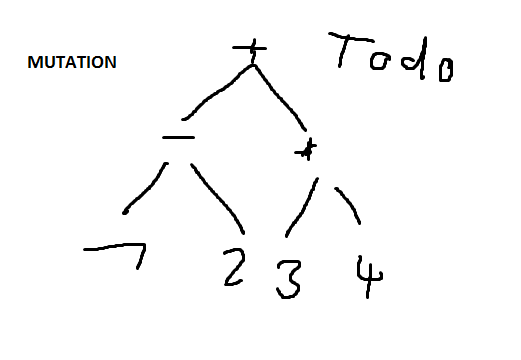
\includegraphics[width=1\textwidth]{img/trees/explain_mutation.png}
	\caption{TODO}
	\label{img:explain_mutation}
\end{figure}

\subsection{TODO Reproduction}
    
    Some good candidates of the last generation can enter the next one without mutation. This is commonly used in genetic programming [todo source].
    Besides, we introduced two additional forms of reproduction:\\
    \begin{itemize}
        \item tes, that are rather close to the origin in the future, without specifically having to reduce the tree-distance between candidates.
        \item Reproduce from 'olymp'. All pareto efficient candidates, including the origin, have a chance to enter the new generation. they are simple and good, its pareto.should be able to give their genes constantly to next gen 
        \item simplify candidates. Either parts of a complete tree gets reduced to the most basic mathematical form possible. Not all trees should be saved in their basic form, as they might have branches with potential for further changes. On the other side, we want simple trees and generally the most basic solution.
    \end{itemize}

\subsection{TODO Genetic Crossover}
    
Candidates can recombine themselves by exchanging their Genes to create children. 

\subsection{TODO Function set, Limitations}

The generated programs consist of operators (todo ?functions?), input values and constant values.

\begin{itemize}
    \item functions / Operators: The set of mathematical operators that make up the program. Possible operators are [TODO $+, -, *$]. 

    Although theoretically all regular functions of regular programming can be used here, loops have been omitted. Although they are a powerful tool in computer science, they lead to severe optimization problems and evaluation problems.
    
    If while-loop is running endlessly, the program can never come to a result and even with a limited number of repetitions the evaluation can take extremely long.
    

    \item Terminals:
    
    Input values: The amount of possible observations in a problem. 
    
    Variables (optional): Randomly chosen constant values. Beside simple values like \tt{True} or \tt{False} mainly numerical constants are selected.

\end{itemize}

Programs can be displayed as a computational tree. TODO image] These are very memory efficient and their components can be easily recognized and divided. 

\subsection{TODO Complexity threshold}


- Complexity

Although fitness is the main criterion, there is often a maximum size that a candidate may not exceed. Complex trees greatly increase the evaluation time. In addition, above a certain level of complexity, no fundamental improvements are expected to solve the problem. The complexity depends mostly on the number of nodes [todo src], but can also depend on other factors such as the depth of the tree.

\subsection{TODO Type consistancy and evaluation safety}

all functions must create working trees